%%%%%%%%%%%%%%%%%%%%%%%%%%%%%%%%%
%% DIFFERENT CRIME SUMSTATS %%%%%
%%%%%%%%%%%%%%%%%%%%%%%%%%%%%%%%%
\begin{table}[H]\caption{Criminal Charges Against Politicians
    Contesting Election: \cnewline Summary Statistics}
  \begin{center}
  \begin{tabular}{l c c  c}\hline\hline
\multicolumn{1}{c}{\textbf{Variable}} & \textbf{Mean}
 & \textbf{(Std. Dev.)} & \textbf{N}\\ \hline
Number of open charges listed on affidavit & 1.606 & (5.181)  & 9685\\
Any Charge & 0.32 & (0.466)  & 9685\\
Corruption & 0.103 & (0.304)  & 9563\\
Violent Crime & 0.113 & (0.317)  & 9563\\
Property Crime & 0.075 & (0.263)  & 9563\\
Civil Disorder & 0.134 & (0.341)  & 9563\\
White Collar Crime & 0.028 & (0.166)  & 9563\\
Libel & 0.051 & (0.221)  & 9563\\
\hline\end{tabular}

  \end{center}
  \label{tab:pol_crimes}
  
  \footnotesize{The table shows the distribution of charges faced by
    politicians seeking election in India. The sample period is
    2003--2017. 2003 is the first year that candidates were required
    to file affidavits showing criminal charges.  Corruption is
    defined as theft from a government office, illegally attempting to
    influence a public servant or an election-related crime. Violent
    crime includes actual or attempted assault, armed robbery,
    homicide, kidnapping or sexual assault.}
\end{table}

%%%%%%%%%%%%%%%%%%%%%%%%%%%%%%%%%
%% CON FIXED EFFECT ROBUSTNESS %%
%%%%%%%%%%%%%%%%%%%%%%%%%%%%%%%%%

\begin{table}[H]\caption{Robustness of main results to constituency
    fixed effects}
  \vspace{1cm}
  \small
  \textbf{Panel A: Effect of Price Shocks on Winning Candidate Characteristics}
  \setlength{\linewidth}{.1cm} \begin{center}
\newcommand{\contents}{\begin{tabular}{l*{5}{c}}
\hline\hline
 & BJP & INC & High School & Age & Log Net Assets \\ 
%PYTHON_HEADER
                    &         (1)   &         (2)   &         (3)   &         (4)   &         (5)   \\
\hline
Price shock$_{-6,-1}$&       0.032   &      -0.049   &       0.061*  &      -2.178** &      -0.213   \\
                    &     (0.045)   &     (0.048)   &     (0.036)   &     (1.067)   &     (0.321)   \\
\hline
N                   &        1905   &        1905   &         682   &         710   &         710   \\
r2                  &        0.58   &        0.52   &        0.73   &        0.70   &        0.64   \\
\hline
\multicolumn{6}{p{\linewidth}}{$^{*}p<0.10, ^{**}p<0.05, ^{***}p<0.01$} \\
\multicolumn{6}{p{\linewidth}}{\footnotesize \tablenote}
\end{tabular} }
\setbox0=\hbox{\contents}
\setlength{\linewidth}{\wd0-2\tabcolsep-.25em} \contents \end{center}

  \newline
  \small \textbf{Panel B: Effect of Price Shock on Criminality by Type
    of Crime}
  \setlength{\linewidth}{.1cm} \begin{center}
\newcommand{\contents}{\begin{tabular}{l*{4}{c}}
\hline\hline
 & \underline{Violent} & \underline{Non-violent} & \underline{Corruption} & \underline{Not Corruption} \\ 
%PYTHON_HEADER
                    &         (1)   &         (2)   &         (3)   &         (4)   \\
\hline
Price shock$_{-6,-1}$&       0.135** &      -0.023   &       0.069   &       0.043   \\
                    &     (0.067)   &     (0.069)   &     (0.058)   &     (0.080)   \\
\hline
N                   &         711   &         711   &         711   &         711   \\
r2                  &        0.58   &        0.61   &        0.58   &        0.60   \\
\hline
\multicolumn{5}{p{\linewidth}}{$^{*}p<0.10, ^{**}p<0.05, ^{***}p<0.01$} \\
\multicolumn{5}{p{\linewidth}}{\footnotesize \tablenote}
\end{tabular} }
\setbox0=\hbox{\contents}
\setlength{\linewidth}{\wd0-2\tabcolsep-.25em} \contents \end{center}

  \newline
  \small \textbf{Panel C: Effect of Price Shock on Election Competitiveness}
  \setlength{\linewidth}{.1cm} \begin{center}
\newcommand{\contents}{\begin{tabular}{l*{3}{c}}
\hline\hline
 & \underline{Incumbent} & \underline{Turnout} & \underline{ENOP} \\ 
%PYTHON_HEADER
                    &         (1)   &         (2)   &         (3)   \\
\hline
Price shock$_{-6,-1}$&      -0.021   &       0.005   &       0.155***\\
                    &     (0.053)   &     (0.008)   &     (0.054)   \\
\hline
N                   &        1409   &        1536   &        1414   \\
r2                  &        0.47   &        0.89   &        0.68   \\
\hline
\multicolumn{4}{p{\linewidth}}{$^{*}p<0.10, ^{**}p<0.05, ^{***}p<0.01$} \\
\multicolumn{4}{p{\linewidth}}{\footnotesize \tablenote}
\end{tabular} }
\setbox0=\hbox{\contents}
\setlength{\linewidth}{\wd0-2\tabcolsep-.25em} \contents \end{center}


  \label{tab:con_fe}
  \footnotesize{These three panels shows the robustness of Tables
    \ref{tab:ed_age}, \ref{tab:winner_violence}, and \ref{tab:eci} in
    the body of the paper to the inclusion of constituency fixed
    effects. All rows and columns are identical to those tables in the
    body of the paper, but include constituency fixed effects.} \small
\end{table}

%%%%%%%%%%%%%%%%%%%%%%%%%%%%%%%%
%% Mean Candidate Criminality %%
%%%%%%%%%%%%%%%%%%%%%%%%%%%%%%%%
\begin{table}[H]\caption{Effect of mineral price shocks on non-winner criminality}
  \newcommand{\tablenote}{The table estimates the impact of a local
    mineral price shock on the criminality of candidates who contested
    election but did not win. Criminality is a candidate-level
    indicator that takes the value one if the candidate is facing
    criminal charges. The dependent variable in Columns 1--3 is the
    mean of this indicator across all candidates contesting election
    in each constituency-year. The dependent variable in Columns 4--6
    is the criminality of the second-place candidate in each
    constituency-year.  The price shock is the change in global mineral prices, weighted by
constituency pre-sample production values of each mineral, calculated
over the five years preceding the given election.%
 Columns 1 and 4 estimate
    Equation~\ref{eq:main} on the full sample with state*year fixed
    effects. Columns 2 and 5 add district fixed effects and Columns 3
    and 6 add constituency fixed effects.  All regressions include state-year fixed effects and constituency
controls for the number of deposits within 10km of a constituency, a
constituency-level mineral dispersion index, and baseline (2001)
values of log constituency population, share of the population living
in rural areas, share of villages with electricity and the per
capita number of primary schools.  Standard errors are robust and
clustered at the district level.%
}
  \small \setlength{\linewidth}{.1cm} \begin{center}
\newcommand{\contents}{\begin{tabular}{l*{6}{c}}
\hline\hline
                    &         (1)   &         (2)   &         (3)   &         (4)   &         (5)   &         (6)   \\
\hline
Price shock$_{-6,-1}$&       0.010   &       0.007   &      -0.002   &       0.005   &      -0.015   &      -0.035   \\
                    &     (0.015)   &     (0.017)   &     (0.022)   &     (0.041)   &     (0.045)   &     (0.070)   \\
\hline State-Year F.E.     & Yes & Yes & Yes & Yes & Yes & Yes  \\ 
 District F.E.       & No  & Yes & No  & No  & Yes & No   \\ 
 Constituency F.E.   & No  & No  & Yes & No  & No  & Yes  \\ 
\hline 
Mean Dep. Var. & 0.19 & 0.19 & 0.18 & 0.28 & 0.28 & 0.30 \\ 
%PYTHON_FOOTER
\hline
N                   &         987   &         985   &         807   &         855   &         848   &         631   \\
r2                  &        0.22   &        0.39   &        0.66   &        0.18   &        0.34   &        0.63   \\
\hline
\multicolumn{7}{p{\linewidth}}{$^{*}p<0.10, ^{**}p<0.05, ^{***}p<0.01$} \\
\multicolumn{7}{p{\linewidth}}{\footnotesize \tablenote}
\end{tabular} }
\setbox0=\hbox{\contents}
\setlength{\linewidth}{\wd0-2\tabcolsep-.25em} \contents \end{center}

  \label{tab:app_mean_crim}
\end{table}

%%%%%%%%%%%%%%%%%%%%%%%%%
%% LAGGED PRICE SHOCKS %%
%%%%%%%%%%%%%%%%%%%%%%%%%

\newpage
\begin{table}[H]\caption{Effect of mineral price shocks on candidate asset
    growth and criminal activity \cnewline Robustness to lagged
    price shocks}
  \label{tab:app_ts_lag}
  \newcommand{\tablenote}{The table shows estimates of the impact
    of mineral wealth shocks on asset growth of elected leaders
    and on new criminal charges against them. Results are analogous
    to those in Table~\ref{tab:ts}, but with the inclusion of lagged
    price shocks.  The dependent variable in columns 1--2 is the change in a
    candidate's log net assets over a single electoral term. The price
    shock is the unanticipated change in mineral wealth in that
    electoral term, defined as the change in the global prices of the
    basket of mineral in each constituency, measured from the first
    year after the politician is elected to the end of the electoral
    term. Column 1 estimates the regression on elected officials
    only. In Column 2, the sample includes winners and runners up from
    the first election, and the price shock is interacted with a
    dummy variable indicating the election winner. Columns 3 and 4 run specifications comparable to
    Columns 1 and 2, where the dependent variable is an indicator for
    whether the politician is facing more criminal charges at the end
    of the electoral term than at the beginning. All regressions include state-year fixed effects and constituency
controls for the number of deposits within 10km of a constituency, a
constituency-level mineral dispersion index, and baseline (2001)
values of log constituency population, share of the population living
in rural areas, share of villages with electricity and the per
capita number of primary schools.  Standard errors are robust and
clustered at the district level.%
}
  \setlength{\linewidth}{.1cm} \begin{center}
\newcommand{\contents}{\begin{tabular}{l*{4}{c}}
\hline\hline
 & \multicolumn{2}{c}{\underline{Change in Assets}} & \multicolumn{2}{|c}{\underline{Change in Crime}} \\ 
%PYTHON_HEADER
                    &         (1)   &         (2)   &         (3)   &         (4)   \\
\hline
Price shock$_{+1,+5}$&       0.267***&      -0.045   &       0.216***&      -0.045   \\
                    &     (0.101)   &     (0.165)   &     (0.062)   &     (0.087)   \\
Price shock$_{+1,+5}$ * Winner&               &       0.302*  &               &       0.244** \\
                    &               &     (0.168)   &               &     (0.100)   \\
Winner              &               &      -0.142   &               &      -0.420** \\
                    &               &     (0.297)   &               &     (0.201)   \\
Price shock$_{-5,-1}$ (lagged)&       0.095   &       0.191** &       0.023   &      -0.010   \\
                    &     (0.103)   &     (0.092)   &     (0.058)   &     (0.070)   \\
Price shock$_{-5,-1}$ (lagged) * Winner&               &      -0.073   &               &       0.021   \\
                    &               &     (0.119)   &               &     (0.081)   \\
\hline
State-Year F.E. & Yes & Yes & Yes & Yes \\ 
\hline 
Mean Dep. Var. & 1.02 & 0.98 & 0.18 & 0.20 \\ 
%PYTHON_FOOTER
\hline
N                   &         448   &         696   &         364   &         629   \\
r2                  &        0.40   &        0.33   &        0.23   &        0.18   \\
\hline
\multicolumn{5}{p{\linewidth}}{$^{*}p<0.10, ^{**}p<0.05, ^{***}p<0.01$} \\
\multicolumn{5}{p{\linewidth}}{\footnotesize \tablenote}
\end{tabular} }
\setbox0=\hbox{\contents}
\setlength{\linewidth}{\wd0-2\tabcolsep-.25em} \contents \end{center}

\end{table}

\newpage
%%%%%%%%%%%%%%%%%%%%%%%%%%%%%%%%%%%%%%%
%% EMPLOYMENT GROWTH / BARTIK SHOCKS %%
%%%%%%%%%%%%%%%%%%%%%%%%%%%%%%%%%%%%%%%
\begin{table}[H]\caption{Effect of employment shocks on candidate
    selection and behavior}
  \vspace{1cm}
  \small
  \textbf{Panel A: Constituency-Level Non-Farm Employment Growth}
  \footnotesize \setlength{\linewidth}{.1cm} \begin{center}
\newcommand{\contents}{\begin{tabular}{l*{5}{c}}
\hline\hline
 & \underline{Crim Winner} & \multicolumn{2}{c}{\underline{Change in Assets}} & \multicolumn{2}{c}{\underline{Change in Crime}} \\ 
%PYTHON_HEADER
                    &         (1)   &         (2)   &         (3)   &         (4)   &         (5)   \\
\hline
Pre-Election Growth &      -0.003   &               &               &               &               \\
                    &     (0.016)   &               &               &               &               \\
Growth in Electoral Term&               &       0.108   &       0.077   &      -0.045   &       0.224***\\
                    &               &     (0.211)   &     (0.136)   &     (0.046)   &     (0.071)   \\
Winner              &               &               &       0.190   &               &       0.031   \\
                    &               &               &     (0.128)   &               &     (0.056)   \\
Winner * Growth in Electoral Term&               &               &       0.029   &               &      -0.245***\\
                    &               &               &     (0.207)   &               &     (0.072)   \\
Constant            &       0.339***&       1.178***&       1.011***&       0.224***&       0.198***\\
                    &     (0.009)   &     (0.085)   &     (0.104)   &     (0.030)   &     (0.047)   \\
\hline
State-Year F.E. & Yes & Yes & Yes & Yes & Yes \\ 
\hline 
Mean Dep. Var. & 0.34 & 1.21 & 1.17 & 0.21 & 0.25  \\ 
%PYTHON_FOOTER
\hline
N                   &        4427   &         213   &         335   &         219   &         349   \\
r2                  &        0.10   &        0.12   &        0.09   &        0.13   &        0.14   \\
\hline
\multicolumn{6}{p{\linewidth}}{$^{*}p<0.10, ^{**}p<0.05, ^{***}p<0.01$} \\
\multicolumn{6}{p{\linewidth}}{\footnotesize \tablenote}
\end{tabular} }
\setbox0=\hbox{\contents}
\setlength{\linewidth}{\wd0-2\tabcolsep-.25em} \contents \end{center}
 \newline

  \newcommand{\tablenote}{The table replicates the main results of the
    paper using shocks to non-farm sector employment instead of
    mineral wealth shocks. The independent variable in Panel A is
    constituency-level non-farm employment growth; in Panel B, it is
    \textit{predicted} non-farm employment growth from a Bartik
    specification. Column 1 shows a regression of a criminal winner
    indicator on employment growth in the period before the
    election. Columns 2 and 3 show regressions of the change in
    candidate assets on employment growth during the candidate's term
    in office. Columns 4 and 5 show regressions of an indicator that
    takes the value one if a candidate has accumulated additional
    criminal charges during the electoral term, on employment growth
    during the candidate's term in office. Columns 2 and 4 are
    restricted to sitting MLAs (i.e. election winners) only; Columns 3
    and 5 include runners-up in the last election as a control
    group. All regressions include state-year fixed effects and the
    standard set of constituency controls. Standard errors are robust
    and clustered at the district level.}
  \small \textbf{Panel B: Bartik-Predicted Constituency-Level Non-Farm Employment Growth}
  \footnotesize \setlength{\linewidth}{.1cm} \begin{center}
\newcommand{\contents}{\begin{tabular}{l*{5}{c}}
\hline\hline
 & \underline{Crim Winner} & \multicolumn{2}{c}{\underline{Change in Assets}} & \multicolumn{2}{c}{\underline{Change in Crime}} \\ 
%PYTHON_HEADER
                    &         (1)   &         (2)   &         (3)   &         (4)   &         (5)   \\
\hline
Bartik Predicted Pre-Election Growth&       0.078   &               &               &               &               \\
                    &     (0.103)   &               &               &               &               \\
Predicted Growth in Electoral Term&               &      -1.309   &      -2.442   &      -0.287   &       0.142   \\
                    &               &     (0.950)   &     (1.584)   &     (0.316)   &     (0.668)   \\
Winner              &               &               &      -0.289   &               &       0.068   \\
                    &               &               &     (0.714)   &               &     (0.301)   \\
Winner * Predicted Growth in Electoral Term&               &               &       1.158   &               &      -0.313   \\
                    &               &               &     (1.694)   &               &     (0.700)   \\
Constant            &       0.308***&       1.757***&       2.056***&       0.329** &       0.227   \\
                    &     (0.039)   &     (0.397)   &     (0.656)   &     (0.138)   &     (0.281)   \\
\hline
State-Year F.E. & Yes & Yes & Yes & Yes & Yes \\ 
\hline 
Mean Dep. Var. & 0.34 & 1.21 & 1.17 & 0.21 & 0.25 \\ 
%PYTHON_FOOTER
\hline
N                   &        4427   &         213   &         335   &         219   &         349   \\
r2                  &        0.10   &        0.13   &        0.10   &        0.13   &        0.12   \\
\hline
\multicolumn{6}{p{\linewidth}}{$^{*}p<0.10, ^{**}p<0.05, ^{***}p<0.01$} \\
\multicolumn{6}{p{\linewidth}}{\footnotesize \tablenote}
\end{tabular} }
\setbox0=\hbox{\contents}
\setlength{\linewidth}{\wd0-2\tabcolsep-.25em} \contents \end{center}

  \label{tab:app_ec_growth_bartik}
\end{table}

\newpage
%%%%%%%%%%%%%%%%%%%%%%%%%%%%%%%%%%%%%
%% RAINFALL SHOCKS ON ALL OUTCOMES %%
%%%%%%%%%%%%%%%%%%%%%%%%%%%%%%%%%%%%%
\begin{table}[H]\caption{Effect of rainfall shocks on candidate
    selection and behavior}
  \newcommand{\tablenote}{The table replicates the main results of the
    paper using precipitation shocks instead of mineral wealth shocks.
    Column 1 shows a regression of a criminal winner indicator on
    rainfall in the year before the election. Column 2 uses average
    rainfall in the five years before the election.  Columns 3 and 4
    show regressions of the change in candidate assets on average
    rainfall during the candidate's term in office. Columns 5 and 6
    show regressions of an indicator that takes the value one if a
    candidate has accumulated additional criminal charges during the
    electoral term, on average rainfall during the candidate's term in
    office. Columns 3 and 5 are restricted to sitting MLAs
    (i.e. election winners) only; Columns 4 and 6 include runners-up
    in the last election as a control group.  Rainfall in each year is
    measured as total rainfall in the month of monsoon arrival.  All
    regressions include state-year fixed effects and the standard set
    of constituency controls. Standard errors are robust and clustered
    at the district level.
  }  \small
  \setlength{\linewidth}{.1cm} \begin{center}
\newcommand{\contents}{\begin{tabular}{l*{6}{c}}
\hline\hline
 & \multicolumn{2}{c}{\underline{Criminal Winner}} & \multicolumn{2}{c}{\underline{Change in Assets}} & \multicolumn{2}{c}{\underline{Change in Crime}} \\ 
%PYTHON_HEADER
                    &         (1)   &         (2)   &         (3)   &         (4)   &         (5)   &         (6)   \\
\hline
Precip. Year Before Election&       0.001   &               &               &               &               &               \\
                    &     (0.009)   &               &               &               &               &               \\
Precip. 5 Years Before Election&               &      -0.017   &               &               &               &               \\
                    &               &     (0.019)   &               &               &               &               \\
Precip. During Electoral Term&               &               &       0.159   &       0.190   &      -0.014   &       0.108   \\
                    &               &               &     (0.223)   &     (0.205)   &     (0.099)   &     (0.109)   \\
Winner              &               &               &               &       0.194** &               &      -0.052   \\
                    &               &               &               &     (0.084)   &               &     (0.041)   \\
Precip. During Term * Winner&               &               &               &       0.150   &               &      -0.023   \\
                    &               &               &               &     (0.161)   &               &     (0.081)   \\
Constant            &       0.306***&       0.307***&       1.098***&       0.949***&       0.181***&       0.247***\\
                    &     (0.006)   &     (0.005)   &     (0.058)   &     (0.064)   &     (0.026)   &     (0.036)   \\
\hline
State-Year F.E. & Yes & Yes & Yes & Yes & Yes & Yes \\ 
\hline 
Mean Dep. Var. & 0.31 & 0.31 & 1.08 & 1.03 & 0.18 & 0.20 \\ 
%PYTHON_FOOTER
\hline
N                   &        9274   &        9274   &         356   &         596   &         361   &         612   \\
r2                  &        0.13   &        0.13   &        0.19   &        0.15   &        0.17   &        0.13   \\
\hline
\multicolumn{7}{p{\linewidth}}{$^{*}p<0.10, ^{**}p<0.05, ^{***}p<0.01$} \\
\multicolumn{7}{p{\linewidth}}{\footnotesize \tablenote}
\end{tabular} }
\setbox0=\hbox{\contents}
\setlength{\linewidth}{\wd0-2\tabcolsep-.25em} \contents \end{center}

  \label{tab:app_precip}
\end{table}

%%%%%%%%%%%%%%%%%%%%%%%
%% ROBUSTNESS TABLES %%
%%%%%%%%%%%%%%%%%%%%%%%
\newpage
\begin{table}[H]\caption{Effect of mineral price shocks on winning candidate
    criminality \cnewline
    Alternate deposit definitions}
  \label{tab:app_deps_only}
  \newcommand{\tablenote}{ This table estimates the impact of a
    local mineral price shock on the criminality of the local
    elected leader, with specifications parallel to those in Table
    \ref{tab:winner_crim}. The price shock variable is a weighted
    sum of global price shocks to the minerals present in a
    constituency. The dependent variable is an indicator that takes
    the value one if the local election winner is facing criminal
    charges.  Columns 1 through 3 define price shocks using mineral
    deposits strictly within constituency boundaries, under
    different fixed effect specifications. In contrast,
    Table~\ref{tab:winner_crim} weights price shocks using
    proximity to deposits that are close to constituencies.
    Columns 4 through 6 weight price shocks with the number of
    mineral deposits in a constituency, irrespective of whether
    production is reported in that constituency, under different
    fixed effect specifications. In contrast,
    Table~\ref{tab:winner_crim} uses pre-sample mineral output
    values as weights.  Sample size is lower than Table
    \ref{tab:winner_crim} as some constituencies are close to
    deposits but do not contain deposits. All regressions include state-year fixed effects and constituency
controls for the number of deposits within 10km of a constituency, a
constituency-level mineral dispersion index, and baseline (2001)
values of log constituency population, share of the population living
in rural areas, share of villages with electricity and the per
capita number of primary schools.  Standard errors are robust and
clustered at the district level.%
}
  \setlength{\linewidth}{.1cm} \begin{center}
\newcommand{\contents}{\begin{tabular}{l*{6}{c}}
\hline\hline
 & \multicolumn{3}{c}{\underline{Exact Deposit Locations}} & \multicolumn{3}{c}{\underline{Deposits Only}} \\ 
%PYTHON_HEADER
                    &         (1)   &         (2)   &         (3)   &         (4)   &         (5)   &         (6)   \\
\hline
Price shock$_{-6,-1}$&       0.131***&       0.107** &       0.118** &       0.040** &       0.038** &       0.051*  \\
                    &     (0.039)   &     (0.041)   &     (0.056)   &     (0.016)   &     (0.016)   &     (0.028)   \\
\hline State-Year F.E. & Yes & Yes & Yes & Yes & Yes & Yes \\ 
District   F.E.     & No  & Yes & No & No  & Yes & No \\ 
Constituency   F.E. & No  & No  & Yes & No  & No  & Yes \\ 
\hline 
Mean Dep. Var. & 0.33 & 0.33 & 0.32 & 0.30 & 0.30 & 0.30 \\ 
%PYTHON_FOOTER
\hline
N                   &         628   &         625   &         484   &        3280   &        3270   &        1905   \\
r2                  &        0.18   &        0.39   &        0.69   &        0.13   &        0.25   &        0.66   \\
\hline
\multicolumn{7}{p{\linewidth}}{$^{*}p<0.10, ^{**}p<0.05, ^{***}p<0.01$} \\
\multicolumn{7}{p{\linewidth}}{\footnotesize \tablenote}
\end{tabular} }
\setbox0=\hbox{\contents}
\setlength{\linewidth}{\wd0-2\tabcolsep-.25em} \contents \end{center}

\end{table}

\newpage
\begin{landscape}
  \begin{table}[H]\caption{Effect of price shocks on winning candidate
      criminality \cnewline Alternate price shock definitions}
    \label{tab:app_alt_pshock_regs}
    \newcommand{\tablenote}{ This table estimates the impact of a
      local mineral price shock on the criminality of the local
      elected leader, under alternate price shock
      definitions. The price shock is the change in global mineral prices, weighted by
constituency pre-sample production values of each mineral, calculated
over the five years preceding the given election.%
 The dependent variable is an
      indicator that takes the value one if the local election winner
      is facing criminal charges. Column 1 weights mineral deposits
      based on baseline district-level mineral output measured from 1990--2003,
      instead of 1990--2013. Column 2 defines the price shock from 5
      years before the election date to the present date (as opposed
      to Table \ref{tab:winner_crim} which uses 6 years before to 1
      year before). Column 3, 4 and 5 define mineral constituencies as
      those with production of at least (3) \$1 in any one year;
      \$50,000 in one year; or (5) \$200,000 in any year. In
      Table~\ref{tab:winner_crim}, the threshold is \$100,000. Column
      6 presents the main specification from
      Table~\ref{tab:winner_crim}, with standard errors clustered at
      the state level. Column 7 shows estimates from a placebo
      specification, where the treatment variable is the change in
      value of mineral deposits in constituencies that report zero
      production, i.e. constituencies with unproductive mineral
      deposits. All regressions include state-year fixed effects and constituency
controls for the number of deposits within 10km of a constituency, a
constituency-level mineral dispersion index, and baseline (2001)
values of log constituency population, share of the population living
in rural areas, share of villages with electricity and the per
capita number of primary schools.  Standard errors are robust and
clustered at the district level.%
 }
    \setlength{\linewidth}{.1cm} \begin{center}
\newcommand{\contents}{\begin{tabular}{l*{7}{c}}
\hline\hline
 & Baseline   & Shock_{-5,0} & Prod above & Prod above & Prod above & State    & Placebo \\ &  1990-2003 &              &  0   &   USD 50k   &  USD 200k  & Clusters & Fixed Effects &  \\ 
%PYTHON_HEADER
                    &         (1)   &         (2)   &         (3)   &         (4)   &         (5)   &         (6)   &         (7)   \\
\hline
Price Shock         &       0.136***&       0.134** &       0.087***&       0.086** &       0.120** &       0.097** &       0.029   \\
                    &     (0.046)   &     (0.054)   &     (0.032)   &     (0.041)   &     (0.048)   &     (0.037)   &     (0.043)   \\
\hline State-Year F.E.      & Yes & Yes & Yes & Yes & Yes & Yes & Yes \\ 
       District-Year F.E.   & Yes & Yes & Yes & Yes & Yes & Yes & Yes \\ 
\hline 
Mean Dep. Var. & 0.35 & 0.33 & 0.32 & 0.34 & 0.34 & 0.33 & 0.25 \\ 
%PYTHON_FOOTER
\hline
N                   &         720   &         948   &        1726   &        1063   &         780   &         946   &         679   \\
r2                  &        0.34   &        0.34   &        0.26   &        0.33   &        0.36   &        0.35   &        0.44   \\
\hline
\multicolumn{8}{p{\linewidth}}{$^{*}p<0.10, ^{**}p<0.05, ^{***}p<0.01$} \\
\multicolumn{8}{p{\linewidth}}{\footnotesize \tablenote}
\end{tabular} }
\setbox0=\hbox{\contents}
\setlength{\linewidth}{\wd0-2\tabcolsep-.25em} \contents \end{center}

  \end{table}
\end{landscape}

\newpage
\begin{landscape}
  \begin{table}[H]\caption{Effect of mineral price shocks on candidate asset
      growth and criminal activity \cnewline Alternate
      price shock definitions}
    \label{tab:app_ts_robust}
    \newcommand{\tablenote}{ The table shows estimates of the impact
      of mineral wealth shocks on asset growth of elected leaders,
      and on new criminal charges against them. Results are analogous
      to those in Table~\ref{tab:ts}, but with alternate definitions
      of price shocks.  The dependent variable in columns 1, 3, 5 and
      7 is the change in a candidate's log net assets over a single
      electoral term. The dependent variable in columns 2, 4, 6 and 8
      is an indicator for whether the politician is facing more
      criminal charges at the end of the electoral term than at the
      beginning The price shock is the unanticipated change in
      mineral wealth in that electoral term, defined as the change in
      the global prices of the basket of mineral in each
      constituency, measured from the first year after the politician
      is elected to the end of the electoral term.  Columns 1 and 2
      show results based strictly on mineral deposits, ignoring
      production data. Columns 3 and 4 define production using all
      years of data. Columns 5 and 6 define mineral constituencies at
      the lower production threshold, and Columns 7 and 8 do so at
      the higher production threshold.  All regressions include state-year fixed effects, district fixed
effects and constituency controls for the number of deposits within
10km of a constituency, a constituency-level mineral dispersion index,
and baseline (2001) values of log constituency population, share of
the population living in rural areas, share of villages with
electricity and the per capita number of primary schools.  Standard
errors are robust and clustered at the district level.%
 }
    \setlength{\linewidth}{.1cm} \begin{center}
\newcommand{\contents}{\begin{tabular}{l*{8}{c}}
\hline\hline
 & Assets & Crime & Assets & Crime & Assets & Crime & Assets & Crime \\ 
%PYTHON_HEADER
                    &         (1)   &         (2)   &         (3)   &         (4)   &         (5)   &         (6)   &         (7)   &         (8)   \\
\hline
Price shock$_{+1,+5}$&       0.279***&       0.190** &       0.331***&       0.141** &       0.256** &       0.220***&       0.222** &       0.212***\\
                    &     (0.105)   &     (0.078)   &     (0.118)   &     (0.067)   &     (0.117)   &     (0.070)   &     (0.100)   &     (0.063)   \\
\hline
State-Year F.E. & Yes & Yes & Yes & Yes & Yes & Yes & Yes & Yes \\ 
\hline 
N                   &         301   &         248   &         291   &         240   &         362   &         290   &         477   &         370   \\
r2                  &        0.43   &        0.29   &        0.43   &        0.24   &        0.41   &        0.24   &        0.37   &        0.24   \\
\hline
\multicolumn{9}{p{\linewidth}}{$^{*}p<0.10, ^{**}p<0.05, ^{***}p<0.01$} \\
\multicolumn{9}{p{\linewidth}}{\footnotesize \tablenote}
\end{tabular} }
\setbox0=\hbox{\contents}
\setlength{\linewidth}{\wd0-2\tabcolsep-.25em} \contents \end{center}

  \end{table}
\end{landscape}

%%%%%%%%%%%%%%%%%%%%%%%%
%% SPATIAL SPILLOVERS %%
%%%%%%%%%%%%%%%%%%%%%%%%
\newpage
\begin{table}[H]\caption{Effect of mineral price shocks on winning
    candidate criminality \cnewline Spatial Spillovers}
  \newcommand{\tablenote}{The table estimates the impact of local
    mineral price shocks on the criminality elected politicians in
    neighboring constituencies.  The dependent variable is the share
    of neighboring constituencies in which the election winner faces
    criminal charges.  The price shock is the average price shock in
    the neighboring constituencies. The row marked ``Price Shock to
    Neighbors'' is the price shock in the reference constituency.  In
    both cases, the price shock is a change in global mineral prices,
    weighted by constituency pre-sample production values of each
    mineral, calculated over the five years preceding the given
    election.  Column 1 estimates Equation~\ref{eq:main} on the full
    sample with state*year fixed effects, with the additional
    neighboring price shock variable. Columns 2 and 3 respectively add
    district and constituency fixed effects. Column 4 shows the marginal effect from a probit
    estimation of a similar specification to that in Column
    1. All regressions include state-year fixed effects and constituency
controls for the number of deposits within 10km of a constituency, a
constituency-level mineral dispersion index, and baseline (2001)
values of log constituency population, share of the population living
in rural areas, share of villages with electricity and the per
capita number of primary schools.  Standard errors are robust and
clustered at the district level.%
 }  \small
  \setlength{\linewidth}{.1cm} \begin{center}
\newcommand{\contents}{\begin{tabular}{l*{4}{c}}
\hline\hline
                    &         (1)   &         (2)   &         (3)   &         (4)   \\
\hline
Price Shock         &       0.163***&       0.194***&       0.202***&       0.118*  \\
                    &     (0.053)   &     (0.059)   &     (0.071)   &     (0.070)   \\
Price Shock to Neighbors&      -0.044   &      -0.052   &      -0.050   &      -0.035   \\
                    &     (0.045)   &     (0.044)   &     (0.051)   &     (0.058)   \\
\hline State-Year F.E.      & Yes & Yes & Yes & Yes \\ 
 District F.E.        & No  & Yes & Yes & No  \\ 
 Constituency F.E.    & No  & No  & Yes & No  \\ 
\hline 
Mean Dep. Var. & 0.33 & 0.33 & 0.33 & 0.33 \\ 
%PYTHON_FOOTER
\hline
N                   &         865   &         862   &         650   &         786   \\
r2                  &        0.37   &        0.57   &        0.75   &               \\
\hline
\multicolumn{5}{p{\linewidth}}{$^{*}p<0.10, ^{**}p<0.05, ^{***}p<0.01$} \\
\multicolumn{5}{p{\linewidth}}{\footnotesize \tablenote}
\end{tabular} }
\setbox0=\hbox{\contents}
\setlength{\linewidth}{\wd0-2\tabcolsep-.25em} \contents \end{center}

  \label{tab:app_spill}
\end{table}

%%%%%%%%%%%%%%%%%%%%%%%%%%%%%%%%%%%%%%%%%%%%
%% ALTERNATE CONTINUOUS CRIME DEFINITIONS %%
%%%%%%%%%%%%%%%%%%%%%%%%%%%%%%%%%%%%%%%%%%%%
\newpage
\begin{table}[H]\caption{Adverse selection and moral hazard tests \cnewline
    Alternate crime definitions}
  \newcommand{\tablenote}{This table tests the robustness of results
    in Tables~\ref{tab:winner_crim} and \ref{tab:ts} to alternate
    definitions of the criminality of the winner. Columns 1 and 2 estimate the impact of local
    pre-election mineral price shocks on the criminality of the local elected
    politician. The dependent variable in Column 1 is the number of
    criminal charges faced by the winner; in Column 2 it is the log of
    the number of criminal charges plus one. Columns 3 and 4 estimate
    the impact of post-election mineral price shocks on the number of
    charges faced by the elected leader in a constituency. These columns
    again show the effect on the number of charges and the log number of charges.
    All columns include state and year fixed effects. Columns 1 and 2
    include district fixed effects. All regressions include state-year fixed effects and constituency
controls for the number of deposits within 10km of a constituency, a
constituency-level mineral dispersion index, and baseline (2001)
values of log constituency population, share of the population living
in rural areas, share of villages with electricity and the per
capita number of primary schools.  Standard errors are robust and
clustered at the district level.%

  } \small \setlength{\linewidth}{.1cm} \begin{center}
\newcommand{\contents}{\begin{tabular}{l*{4}{c}}
\hline\hline
 & \multicolumn{2}{c}{\underline{Adverse Selection}} & \multicolumn{2}{c}{\underline{Moral Hazard (Differences)}} \\  & Num Crime & Log Num Crime & Num Crime & Log Num Crime  \\ 
%PYTHON_HEADER
                    &         (1)   &         (2)   &         (3)   &         (4)   \\
\hline
Price shock$_{-6,-1}$&       0.646***&       0.201***&               &               \\
                    &     (0.172)   &     (0.055)   &               &               \\
Price shock$_{+1,+5}$&               &               &       1.082** &       0.209** \\
                    &               &               &     (0.517)   &     (0.091)   \\
\hline
State-Year F.E. & Yes & Yes & Yes & Yes \\ 
\hline 
Mean Dep. Var. & 1.33 & 0.43 & -0.55 & -0.05 \\ 
%PYTHON_FOOTER
\hline
N                   &         948   &         948   &         364   &         364   \\
r2                  &        0.20   &        0.22   &        0.56   &        0.55   \\
\hline
\multicolumn{5}{p{\linewidth}}{$^{*}p<0.10, ^{**}p<0.05, ^{***}p<0.01$} \\
\multicolumn{5}{p{\linewidth}}{\footnotesize \tablenote}
\end{tabular} }
\setbox0=\hbox{\contents}
\setlength{\linewidth}{\wd0-2\tabcolsep-.25em} \contents \end{center}

  \label{tab:app_crime_alt}
\end{table}



%%%%%%%%%%%%%%%%%%%%%%%%%
%% IRON/COAL EXCLUSION %%
%%%%%%%%%%%%%%%%%%%%%%%%%
\newpage
\begin{landscape}
  \begin{table}[H]\caption{Effect of price shocks on winning candidate
      criminality \cnewline Iron, coal, conflict exclusions}
    \label{tab:app_no_iron_coal_regs}
    \newcommand{\tablenote}{ This table estimates the impact of a
      local mineral price shock on the criminality of the local elected
      leader, excluding certain effects in coal- and iron-producing
      regions. The price shock is the change in global mineral prices, weighted by
constituency pre-sample production values of each mineral, calculated
over the five years preceding the given election.%
 The dependent variable is an
      indicator that takes the value one if the local election winner
      is facing criminal charges. Column 1 calculates price shocks
      with coal deposits excluded; Column 2 excludes iron deposits
      from the price shock, and Column 3 excludes both. Columns 4-6
      drop constituencies entirely if they have (4) a coal deposit,
      (5) an iron deposit, or (6) either a coal or iron deposit. Column
      7 excludes the four states with the greatest Naxalite presence
      (Orissa, Andhra Pradesh, Jharkhand and Chhattisgarh). Column 8
      excludes districts with at least Naxalite conflict-related death
      between 2005--2010.
      All regressions include state-year fixed effects, district fixed
effects and constituency controls for the number of deposits within
10km of a constituency, a constituency-level mineral dispersion index,
and baseline (2001) values of log constituency population, share of
the population living in rural areas, share of villages with
electricity and the per capita number of primary schools.  Standard
errors are robust and clustered at the district level.%
 } \footnotesize
    \setlength{\linewidth}{.1cm} \begin{center}
\newcommand{\contents}{\begin{tabular}{l*{8}{c}}
\hline\hline
                    &         (1)   &         (2)   &         (3)   &         (4)   &         (5)   &         (6)   &         (7)   &         (8)   \\
\hline
Price shock$_{-6,-1}$&       0.100** &       0.142***&       0.128***&       0.118***&       0.171***&       0.178***&       0.129** &       0.163***\\
                    &     (0.040)   &     (0.043)   &     (0.040)   &     (0.045)   &     (0.054)   &     (0.055)   &     (0.057)   &     (0.047)   \\
\hline Price Shock   & No coal & No iron & No coal/iron & No coal & No iron & No coal/iron & All & All \\ 
Constituency Sample  & All     &     All & All          & No coal & No iron & No coal/iron & No Naxalite States & No Naxalite Districts \\ 
State-Year F.E. & Yes & Yes & Yes & Yes & Yes & Yes & Yes & Yes\\ 
\hline 
Mean Dep. Var. & 0.33 & 0.33 & 0.33 & 0.32 & 0.33 & 0.32 & 0.32 & 0.32 \\ 
%PYTHON_FOOTER
\hline
N                   &         863   &         891   &         800   &         766   &         738   &         572   &         633   &         660   \\
r2                  &        0.13   &        0.14   &        0.14   &        0.12   &        0.16   &        0.16   &        0.15   &        0.16   \\
\hline
\multicolumn{9}{p{\linewidth}}{$^{*}p<0.10, ^{**}p<0.05, ^{***}p<0.01$} \\
\multicolumn{9}{p{\linewidth}}{\footnotesize \tablenote}
\end{tabular} }
\setbox0=\hbox{\contents}
\setlength{\linewidth}{\wd0-2\tabcolsep-.25em} \contents \end{center}
 \end{table}
\end{landscape}

%%%%%%%%%%%%%%%%%%%%%%%%%%%%%%
%% FIXED CANDIDATE LOCATION %%
%%%%%%%%%%%%%%%%%%%%%%%%%%%%%%
\newpage
\begin{table}[H]\caption{Effect of price shocks on winning candidate
    criminality \cnewline Fixed candidate location}
  \label{tab:app_fixed_loc}
  \newcommand{\tablenote}{}
  \setlength{\linewidth}{.1cm} \begin{center}
\newcommand{\contents}{\begin{tabular}{l*{4}{c}}
\hline\hline
 & All & Moved $<$ 20km & Moved $<$ 10km & Moved $<$ 5km \\ 
%PYTHON_HEADER
                    &         (1)   &         (2)   &         (3)   &         (4)   \\
\hline
Price shock$_{-6,-1}$&       0.197** &       0.177** &       0.149*  &       0.164*  \\
                    &     (0.079)   &     (0.076)   &     (0.077)   &     (0.091)   \\
\hline
State-Year F.E. & Yes & Yes & Yes & Yes \\ 
\hline 
Mean Dep. Var. & 0.43 & 0.43 & 0.43 & 0.43 \\ 
%PYTHON_FOOTER
\hline
N                   &         294   &         275   &         266   &         254   \\
r2                  &        0.19   &        0.27   &        0.25   &        0.27   \\
\hline
\multicolumn{5}{p{\linewidth}}{$^{*}p<0.10, ^{**}p<0.05, ^{***}p<0.01$} \\
\multicolumn{5}{p{\linewidth}}{\footnotesize \tablenote}
\end{tabular} }
\setbox0=\hbox{\contents}
\setlength{\linewidth}{\wd0-2\tabcolsep-.25em} \contents \end{center}

\end{table}
\begin{adjustwidth}{2cm}{2cm}
  \footnotesize{This table estimates the impact of a local mineral
    price shock on the criminality of the local elected leader (as in
    Table \ref{tab:winner_crim}), but limits the sample to candidates
    who have not changed constituencies from one electoral period to
    the next. We define candidates who have not moved as those for
    whom the constituency centroid is less than a given distance from
    that in the previous election. The mean constituency diameter is
    approximately 45km.  The price shock is the change in global mineral prices, weighted by
constituency pre-sample production values of each mineral, calculated
over the five years preceding the given election.%
 The dependent variable is
    an indicator that takes the value one if the local election winner
    is facing criminal charges. Column 1 includes the full sample of
    candidates that we are able to observe in the previous electoral
    term. Column 2 limits to candidates who have moved less than 20km
    since the previous electoral term. Column 3 limits to candidates
    who have moved less than 10km, and Column 4 to 5km.  All regressions include state-year fixed effects and constituency
controls for the number of deposits within 10km of a constituency, a
constituency-level mineral dispersion index, and baseline (2001)
values of log constituency population, share of the population living
in rural areas, share of villages with electricity and the per
capita number of primary schools.  Standard errors are robust and
clustered at the district level.%
}
\end{adjustwidth}

%%%%%%%%%%%%%%%%%%%%%%%%%%%%%%%%
%% SAMPLE CONSTRUCTION FIGURE %%
%%%%%%%%%%%%%%%%%%%%%%%%%%%%%%%%
\newpage
\begin{figure}[H]\caption{Sample construction}
  \begin{center}
    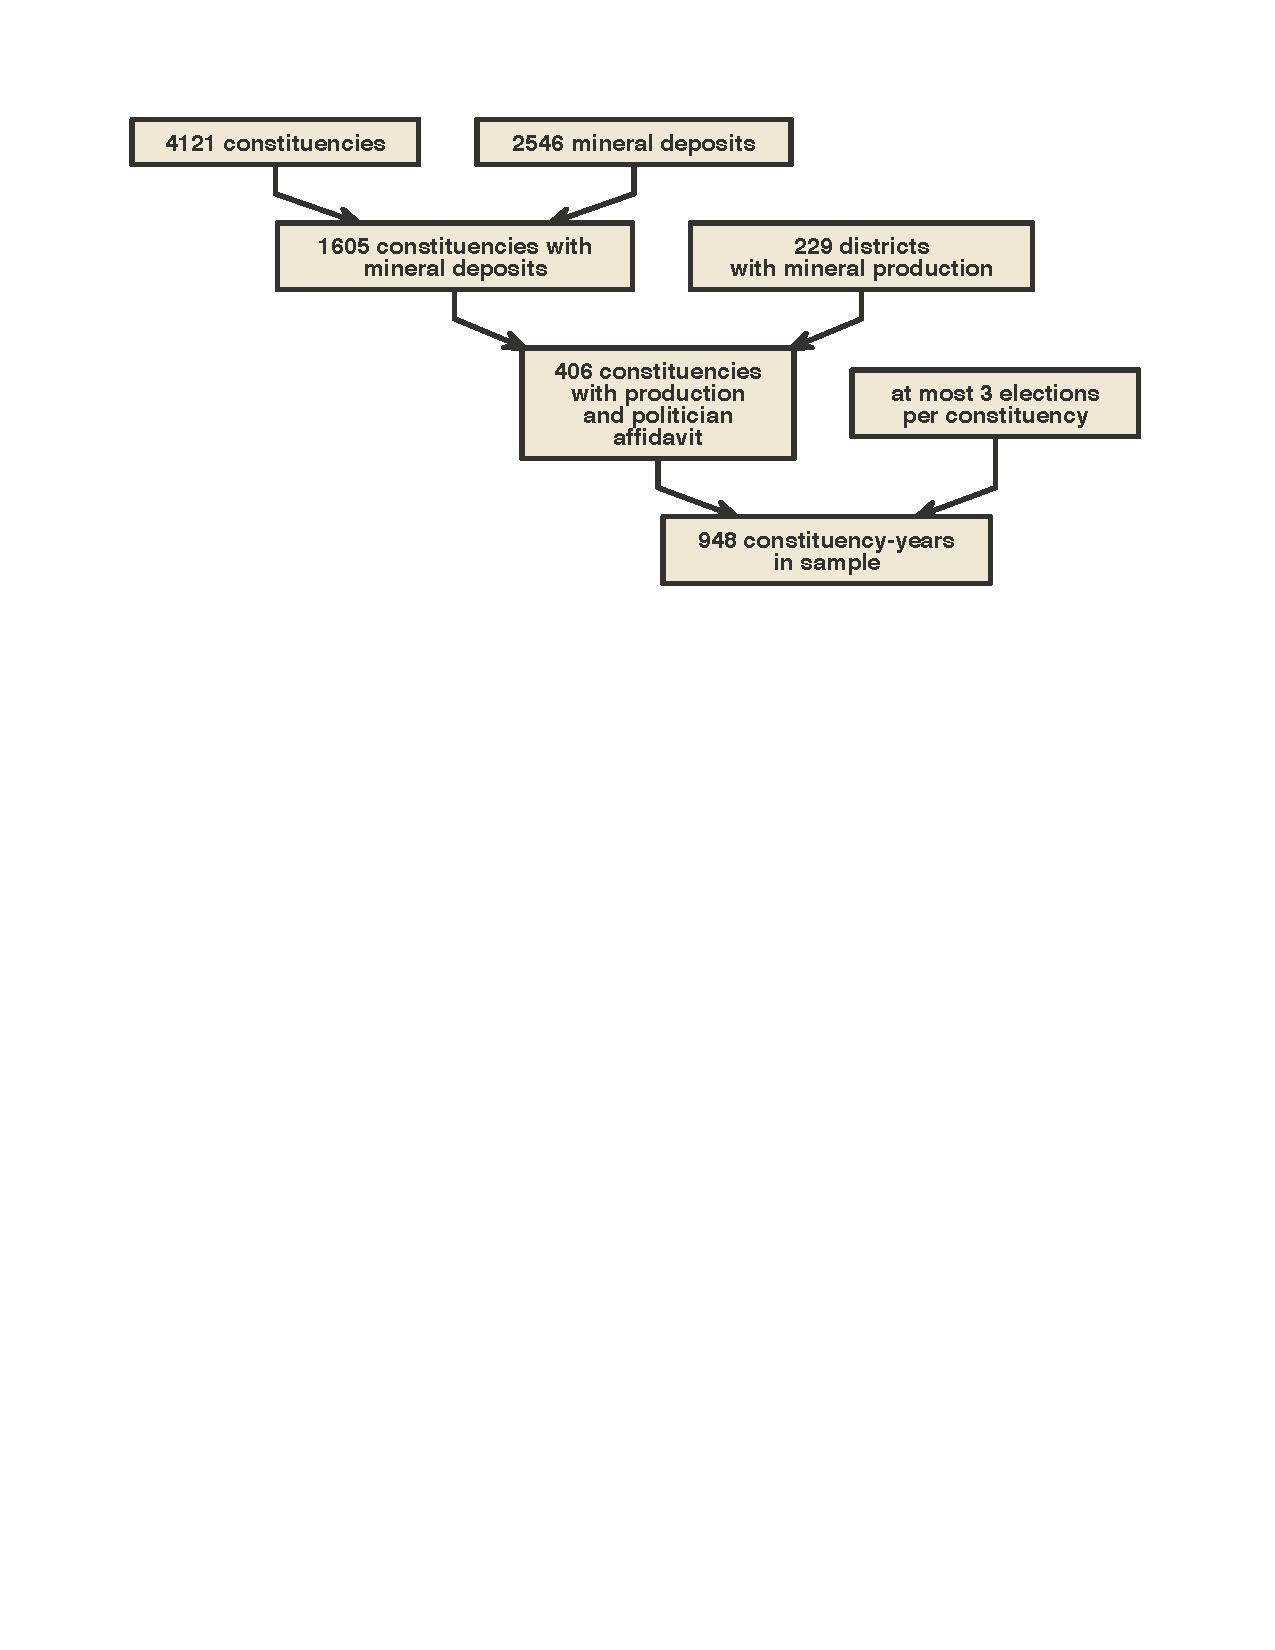
\includegraphics[scale=0.7]{\miningpath/nomnoml}
    \label{fig:app_sample}
  \end{center}
  \footnotesize{The figure describes the process for generating the
    sample of constituencies with valuable mineral deposits, based on
    predelimitation constituencies. The sample consists of 4121
    predelimitation constituencies. These are matched to 2546 mineral
    deposits (Geological Survey of India 2005), and to district-level
    production data (229 districts, Statistics of Mineral Information,
    Indian Bureau of Mines). 1605 constituencies are within 10km of
    mineral deposits, and 406 of these are in districts that report
    production of the same mineral between 1990 and 2013. Each
    constituency has either two or three elections in the sample
    period, leading to a main sample size in
    Table~\ref{tab:winner_crim} of 948 constituency-years.}
\end{figure}  


%%%%%%%%%%%%%%%%%%%%%%%%%%%%%%%%
%% SAMPLE CONSTRUCTION FIGURE %%
%%%%%%%%%%%%%%%%%%%%%%%%%%%%%%%%
\newpage
\begin{figure}[H]\caption{Moral Hazard Estimates: Robustness to Attrition}
  \begin{center}
    
    \small
    
    \textbf{Panel A: Log Asset Growth}
    
    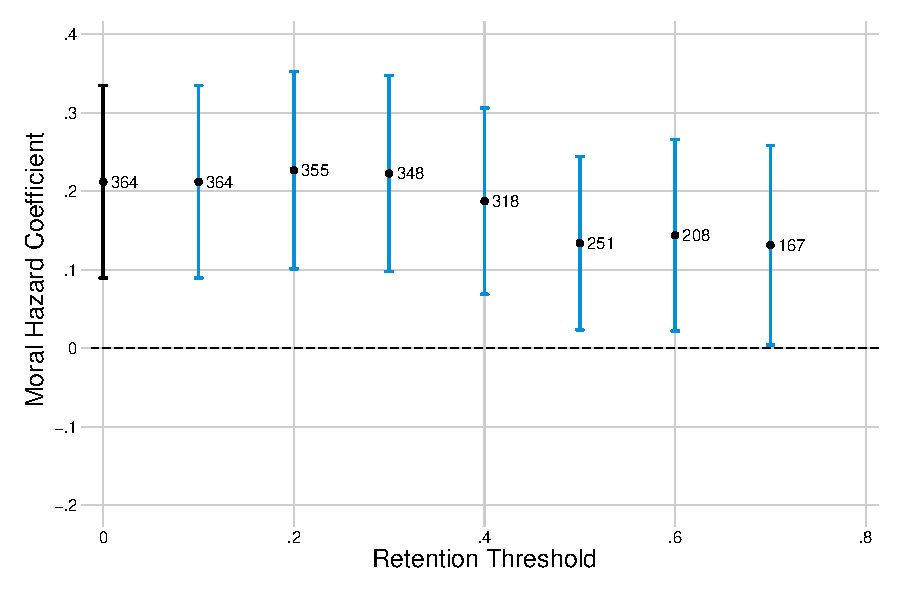
\includegraphics[scale=0.80]{\miningpath/mh_asset_robust}
    
    \label{fig:app_mh_attrition}

    \textbf{Panel B: Criminal Charge Growth}
    
    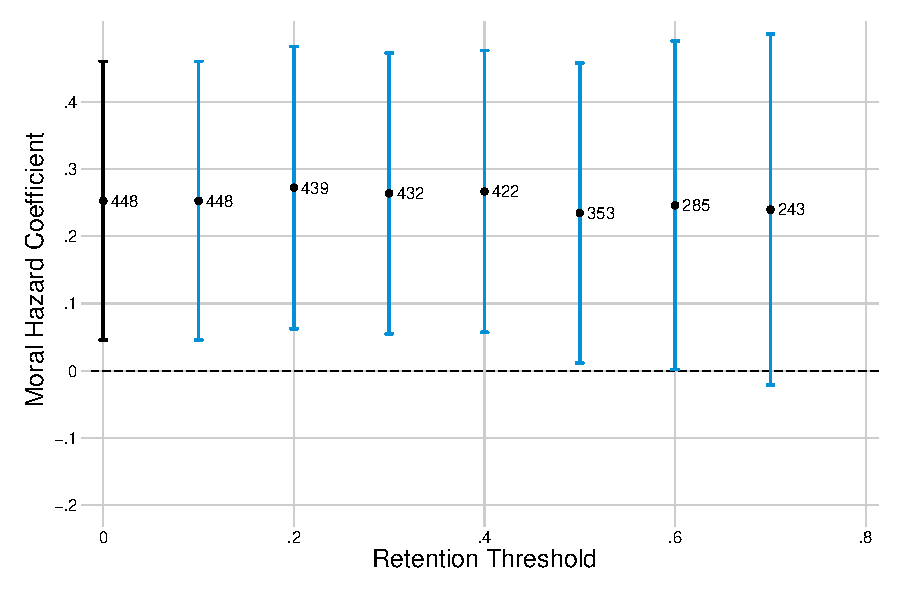
\includegraphics[scale=0.80]{\miningpath/mh_crime_robust}
    
  \end{center}
  \footnotesize{The figure shows alternate estimations of the moral
    hazard effects in Columns 1 and 4 of Table~\ref{tab:ts}. The
    retention threshold on the X axis is a state-election-level variable
    defined as the minimum share of constituencies in that election for which
    we were able to observe the winner again in the following
    election. The estimate at X=0 is the estimate in the paper. The
    remaining estimates increasingly shrink the sample to a set of
    elections where candidate attrition is less of a concern. The aim
    is to show the sensitivity of the estimates to potential
    attrition. The outcome variable is candidate change in
    assets in Panel A and change in criminal charges in Panel B. The
    regression estimate shows the effect of a change in local mineral
    wealth that occurs after an election on the change in assets or
    crime of the political representative serving that
    constituency. The points show the point estimate of each
    estimation along with the sample size.
  }
\end{figure}  

